\def\pathToRoot{.}
\documentclass[a4paper, 12pt]{article}

\usepackage[utf8]{inputenc}
\usepackage{ifthen}
\usepackage{xparse}
\usepackage{scrextend}
\usepackage{setspace}
\usepackage{verbatim}
\usepackage{color}
\usepackage[inline]{enumitem}
\usepackage[colorlinks=true, linkcolor=black, citecolor=black]{hyperref}

\usepackage{tikz}
\usepackage{pgfplots}
\usepackage{bbold}
\usepackage{listings}

\usepackage{subcaption}

\usepackage{amsmath}
\usepackage{amssymb}
\usepackage{latexsym}
\usepackage{hyperref}
\usepackage{cleveref}

\definecolor{gray}{rgb}{0.2,0.2,0.2}

\pagenumbering{arabic}


\usepackage[a4paper, left=2cm, top=2cm, right=2cm, bottom=2cm]{geometry}

\usepackage{multirow}
\usepackage{fancyvrb}

\newcommand{\vect}[1]{\boldsymbol{#1}}

\newcounter{exerciseCounter}
\setcounter{exerciseCounter}{0}

\newcommand{\exerciseNumber}{\sheetnumber.\arabic{exerciseCounter}}

\setenumerate{label=\alph*)}

% Sheet Header
\newcommand{\exercisehead}[3]
{
    \def\sheetnumber{#1}
    \begin{center}
        \begin{minipage}{0.45\linewidth}
            \textsc{Universität des Saarlandes}
            \par
           Prof. Dr. Dietrich  Klakow
           \par
           Lehrstuhl für Signalverarbeitung
           \par
           NNIA Winter Term 2019/2020
        \end{minipage}
        \begin{minipage}{0.45\linewidth}
            \begin{flushright}
               
\includegraphics[width=0.30\linewidth]{headers/lsv_logo.jpg}
            \end{flushright}
        \end{minipage}
        \vspace{5pt}
        \hrule
        \vspace{12pt}
        \doublespacing
        {
            \LARGE
            \textbf{Exercise Sheet #1}
        }
        \par
        {
            \large
            #2
        }
        \par
        \ifdefined\issolution
        \textit{(Solutions)}
        \else
        \fi
        
    \textbf{Deadline: #3}

    \end{center}
    \vspace{2pt}
    \hrule
    \vspace{12pt}
}

% Exercise environment
\NewDocumentEnvironment{exercise}{oo}
{
	\refstepcounter{exerciseCounter}
	\par
	\vspace{12pt}
    \noindent
    \textbf{Exercise \exerciseNumber \  - #1}\IfNoValueF{#2}{\hfill(#2 points)}
	\vspace{12pt}
	\par
	\begin{addmargin}[12pt]{0pt}
}
{
    
	\end{addmargin}
	\par
	\vspace{12pt}
}

% Solution environment
\newenvironment{solution}
{
		\ifthenelse{\isundefined{\issolution}}
		{
			\comment
		}
		{
			\par
			\color{gray}
			\vspace{6pt}
			\textit{Solution \exerciseNumber}
			\par
			\begin{addmargin}[30pt]{0pt}
		}
}
{
		\ifthenelse{\isundefined{\issolution}}
		{
		}
		{
			\end{addmargin}
			\par
			\vspace{12pt}
		}
}



\def\issolution{}

\begin{document}

% {Sheet number}{headline}{deadline}
\exercisehead{9}{\small Philip Georgis [s8phgeor], Pauline Sander [s8pasand], Vilém Zouhar [vizo00001] }{26. 1. 2021}

\section*{Exercises}

\newcommand{\TODO}[1]{\textcolor{red}{TODO:#1}}

\begin{exercise}[CNN Architecture][1 + 1 = 2]

\begin{enumerate}
    
    \item The first convolutional layer of Alex Krizhevsky's AlexNet image recognition network has 96 kernels of size 11x11, with a stride of 4 and padding of 0.  The inputs to this layer were 227x227 pixel three-color images with bias terms.  Compute how many parameters this first convolutional layer of AlexNet has.
    
    \item What is the difference between max pooling and average pooling? Is there a reason why we would prefer one over another for a given problem? If so, explain why, giving concrete examples where possible. (3-5 sentences)
    
\end{enumerate}

\end{exercise}


\begin{solution}
   \begin{enumerate}
       \item Because of sparse connections and tied weights the number of weights per kernel is $11*11*3$, plus one bias parameter. The total number of parameters then is $(11*11*3+1)*96 = 34,944$. 
       \item Pooling is a way to downsample feature maps (say 9x9 to 3x3 with 3x3 filters and stride 3). Both for average pooling and max pooling divide the original map in `pools' of the same size (in this case 9 pools of 3x3). We then take (1) the maximal value in the pool (with max pooling), or (2) the average of all values in the pool (with average pooling) to represent the pool in the downsampled map. Max pooling is often preferred for tasks such as object recognition because the output is invariant and independent of the orientation of the input.
   \end{enumerate}
\end{solution}


\begin{exercise}[CNN for NLP][0.5 + 1 + 0.5 = 2]

Discuss the application of CNN on language sequences by researching on Internet:
\begin{enumerate}
	\item How do we define the input?
	\item What happens to the input during the forward pass? A sketch + 4-5 sentences.
	\item What benefit does it have over simple fully connected NNs?
\end{enumerate}
\end{exercise}


\begin{solution}
\begin{enumerate}
   \item The input is dependent on the task and not that much on whether we are doing CNN or RNN. If we want to process a sequence (length $S$) of word embeddings (dimension $D$), we may with to store them in a tensor $S\times D$ or $S\times 1 \times D$. In the second case, the number of channels is the dimensionality of the embedding, while in the first one, they are flattened. If we are doing a separate convolution per every channel, then the output shapes are going to be vastly different. Both approaches are shown to work.
   \item Assume that we are doing machine translation. Then the encoding step can be done with CNNs in the previous manner. In the following example assume we have a sequence of length 4, which we pad so that the output ``sequence'' has the same length. Horizontal stride is 1, vertical stride is 3. This means that we are computing 3-gram representations of only a part of the embedding vectors. Embeddings in this case have length 8 (much lower than what would normally be used).
   
   If we wish to have a single vector representation of the whole sequence, we can run a (bi)RNN.
   
   \begin{figure}[ht]
        \centering
        \hspace{2.5cm}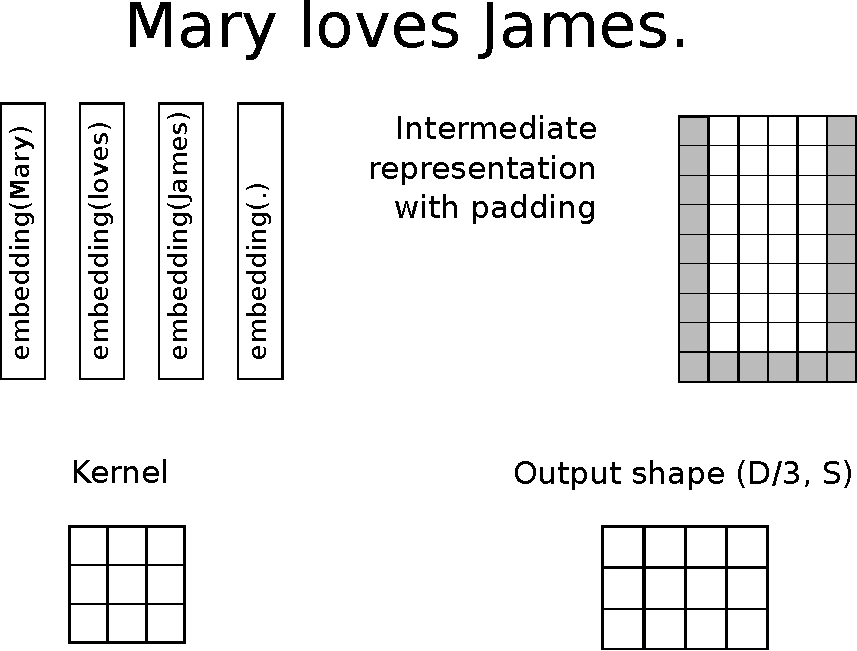
\includegraphics[width=0.6\linewidth]{img/cnn_sketch.pdf}
   \end{figure}
   
   In general the dimensionality decreases (unless it's not padded properly), but we often use multiple sets of kernels, so we increase the channel dimensions.
   
   \item It forces the network to generalize more. In the case where we want to make a variable length representation of a sequence, it would not even make sense to use fully connected dense layers. The network would need to be scaled dynamically according to the input sequence length. For CNN and especially for RNNs, this is not an issue. This could be fixed by padding the sequence by some zero vectors to a fixed maximum length, but even then the parameters of the dense layers would be fixed for a given position.
   
   The number of parameters is also greatly reduced.
\end{enumerate}
\end{solution}

\end{document}
